\section{Financial Performance Highlights}
\begin{figure}[h]
    \centering
    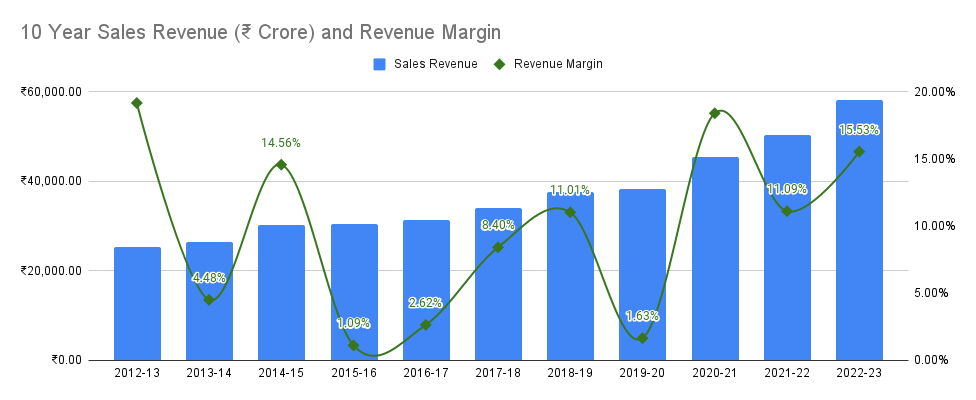
\includegraphics[width=0.9\textwidth]{images/10 Year Sales Revenue.png}
    \caption{10 Year Sales Revenue (\rupee  Crore) and Revenue Margin}
    \label{fig:your_svg_image}
  \end{figure}
In the fiscal year 2022-23, Hindustan Unilever Limited (HUL) exhibited robust financial performance, achieving significant milestones and reinforcing its position as a leader in the Fast Moving Consumer Goods (FMCG) sector. The company witnessed an impressive growth trajectory, adding \rupee8,000 crores to its turnover, which reached \rupee58,154 crores. This remarkable achievement marked a substantial increase from the previous fiscal year, showcasing a growth rate of 16\%. HUL's top line and underlying volumes experienced substantial expansions, registering growth rates of 16\% and 5\%, respectively. Notably, this growth outpaced the market, with over 75\% of the business securing increased market shares.

The profitability metrics also demonstrated a commendable performance, with Profit After Tax (PAT) standing at \rupee9,900 crores, reflecting a noteworthy 13\% increase. The Earnings Per Share (EPS) reached \rupee42 per share, highlighting the company's commitment to delivering value to its shareholders. HUL's efficient capital utilization was evident in its impressive Return on Capital Employed (ROCE) of over 100\%, emphasizing the company's ability to generate substantial returns from its invested capital. Additionally, HUL generated a substantial cash inflow of more than \rupee12,500 crores from its operations, further strengthening its financial position.

\begin{figure}[h]
    \centering
    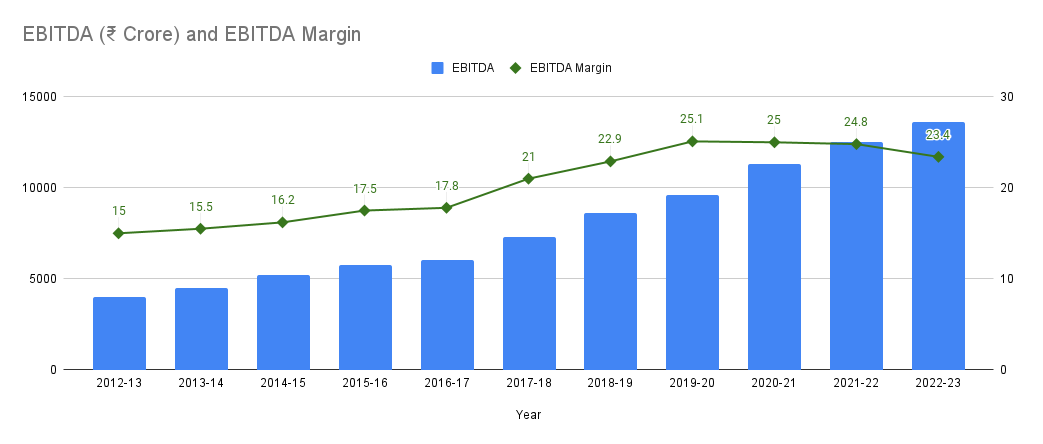
\includegraphics[width=0.9\textwidth]{images/EBITDA.png}
    \caption{EBITDA (\rupee Crore) and EBITDA Margin}
    \label{fig:EBITDA}
  \end{figure}

The trajectory of HUL's turnover over the past decade, as depicted in the provided data, showcases a consistent upward trend, culminating in the noteworthy \rupee58,154 crores in FY'23. Similarly, the Earnings Before Interest, Taxes, Depreciation, and Amortization (EBITDA) reflected a positive trajectory, reaching \rupee13,632 crores in FY'23, with a healthy margin of 23.4\%.

Overall, HUL's financial performance in FY'23 not only demonstrated robust growth in turnover and profitability but also underscored the company's ability to outpace market trends, efficiently utilize capital, and generate substantial cash flows, positioning itself as a powerhouse in the FMCG industry.


\section{Company Analysis}

Hindustan Unilever Limited (HUL), a leading multinational consumer goods company in India, boasts a remarkable track record of growth and innovation. With a strong presence in over 15 categories, HUL is a category leader in over 85\% of its business, showcasing its dominance in the Indian consumer goods market. The company's diverse portfolio includes over 50 brands, with 16 of them generating over \rupee10 billion in turnover each. HUL's commitment to innovation is evident in its five digital-first brands, which cater to the evolving needs of tech-savvy consumers.

In FY'23, HUL achieved an impressive turnover of \rupee58,154 crores, reflecting its strong market position and ability to adapt to changing consumer trends. The company's market capitalization stands at a robust \rupee6 lakh crores, demonstrating its investor confidence and growth potential. With over 21,000 employees, HUL plays a significant role in India's employment landscape.

HUL's EBITDA margin of 23.4\% in FY'23 highlights its operational efficiency and cost management capabilities. The company's extensive distribution network of over 9 million outlets ensures that its products reach every corner of the country, contributing to its widespread market presence. Over the past 20 years, HUL has achieved a remarkable CAGR of 9.26\%, underscoring its consistent growth trajectory.

Looking ahead, HUL remains committed to its vision of making sustainable living a habit. With its strong brand portfolio, innovative products, and robust financial performance, HUL is well-positioned to maintain its leadership position in the Indian consumer goods market and continue to drive positive change in the lives of millions of Indian consumers.

\subsection{Market Share}
\begin{figure}[h]
    \centering
    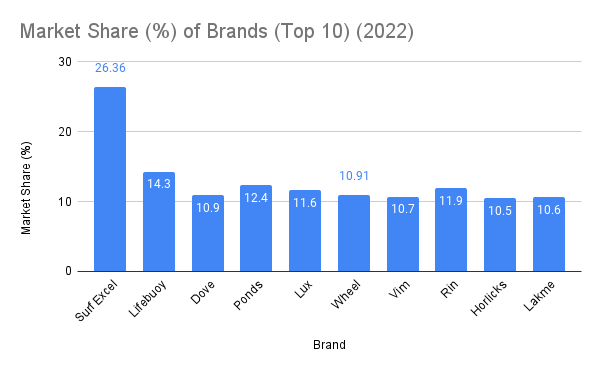
\includegraphics[width=0.9\textwidth]{images/Market Share.png}
    \centering
    \caption{Market Share (\%) of Brands (Top 10) (2022)}
    \label{fig:Market Share}
  \end{figure}
Hindustan Unilever Limited (HUL) boasts a diverse portfolio of leading brands in the Indian market. Among them, Surf Excel dominates with a substantial 26.36\% market share, reflecting its strong presence in the detergent segment. Lifebuoy, a renowned hygiene brand, follows with 14.3\%, emphasizing its significant role in health and well-being. Dove, Ponds, Lux, Wheel, Vim, Rin, Horlicks, and Lakme contribute to HUL's market dominance, each holding substantial market shares ranging from 10.5\% to 12.4\%. This diversified brand landscape underscores HUL's strategic position across various consumer segments, from personal care and hygiene to food and cosmetics.

\subsection{Segment-wise Revenue Contribution (FY'23)}

\begin{figure}[h]
    \centering
    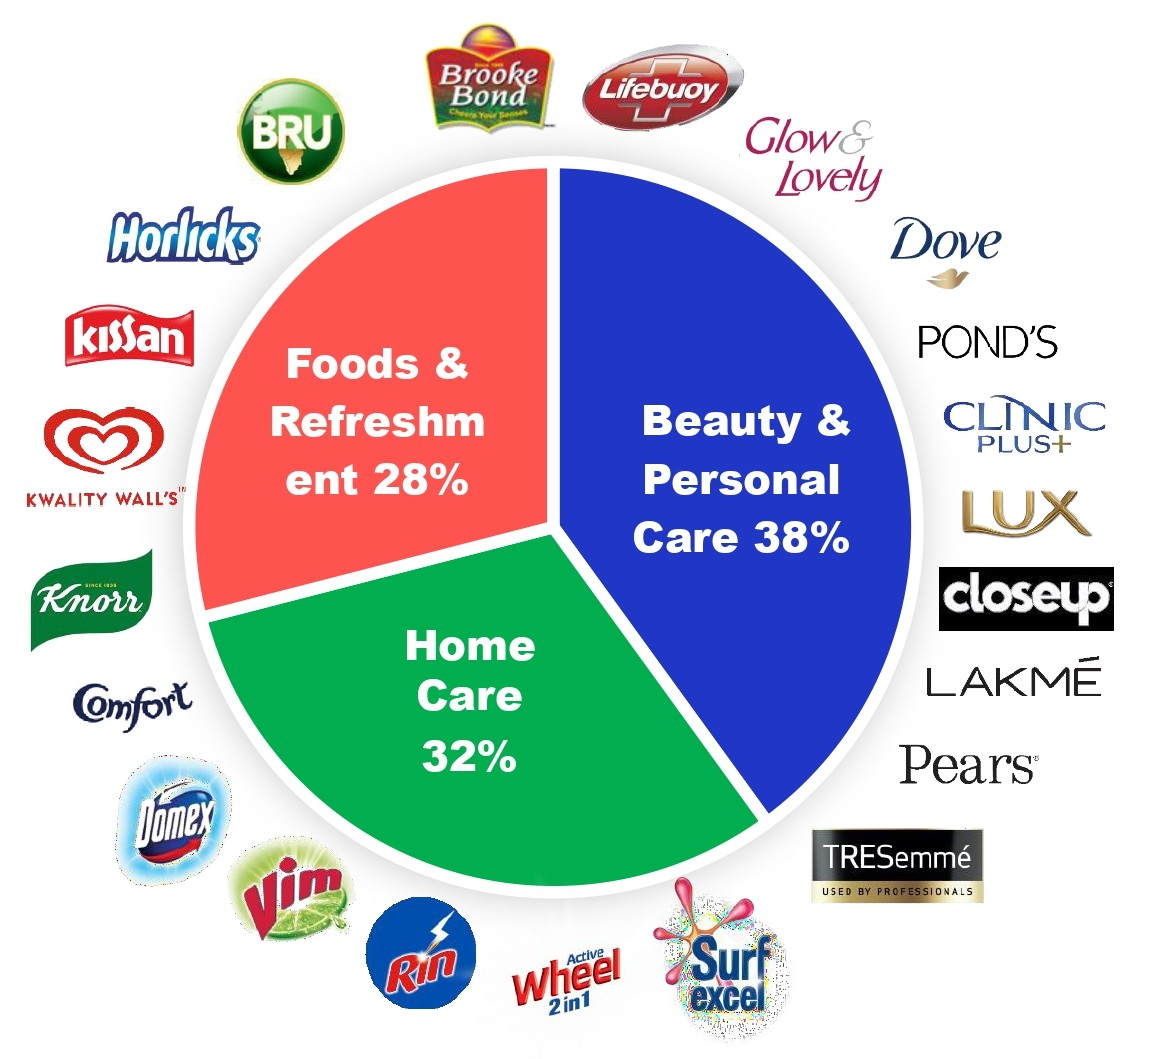
\includegraphics[width=0.9\textwidth]{images/Contri.jpg}
    \centering
    \caption{Revenue Contribution \% \\(Contribution \% based on FY’23 Segment Revenue, excludes others
    )}
    \label{fig:RevContri}
  \end{figure}
\subsubsection{Beauty \& Personal Care (38\%):}
This substantial share underscores the significance of HUL's personal care brands, such as Dove, Lifebuoy, and Lux, in meeting consumer demands for skincare, hygiene, and grooming.

\subsubsection{Home Care (32\%):}
With brands like Surf Excel, Rin, and Vim, HUL's Home Care segment plays a crucial role in addressing consumers' needs for effective and reliable household cleaning products.

\subsubsection{Foods \& Refreshment (28\%):}
The Foods \& Refreshment segment, including brands like Kwality Wall's and Lipton, contributes significantly, emphasizing HUL's presence in the food and beverage sector, aligning with diverse consumer preferences.


\subsection{BCG Matrix}
\begin{figure}[h]
    \centering
    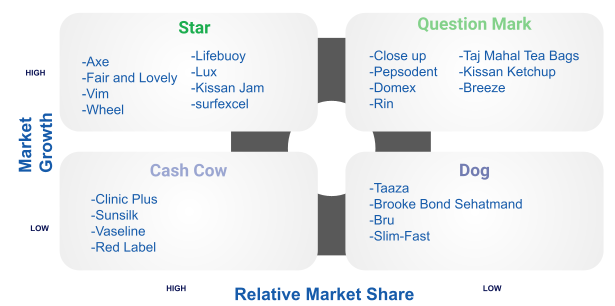
\includegraphics[width=0.9\textwidth]{images/BCG Matrix.png}
    \caption{BCG Matrix}
    \label{fig:BCG Matrix}
  \end{figure}

Hindustan Unilever Limited (HUL) employs the BCG Matrix, a strategic management tool, to analyze and categorize its product portfolio based on market share and market growth. The matrix classifies products into four categories: Question Mark, Star, Dog, and Cash Cow.

\subsection*{Question Mark:
}Products like Close Up, Pepsodent, Domex, Rin, Taj Mahal Tea Bags, Kissan Ketchup, and Breeze fall into this category. These are characterized by a low market share in high-growth markets, representing opportunities for expansion and increased market share. HUL may need to invest and strategize carefully to turn these products into Stars or Cash Cows.

\subsection*{Star:}
Star products, including Lifebuoy, Lux, Kissan Jam, Surf Excel, Axe, Fair and Lovely, Vim, and Wheel, have a high market share in high-growth markets. These are leaders in their respective categories and contribute significantly to HUL's revenue. Continuous investment and strategic focus are essential to maintain and enhance their market position.

\subsection*{Dog:}
Dog products have a low market share in low-growth markets. Taaza, Brooke Bond Sehatmand, Bru, and Slim-Fast fall into this category. These products may not be contributing significantly to growth, and strategic decisions need to be made about their future in the portfolio.

\subsection*{Cash Cow:}
Clinic Plus, Sunsilk, Vaseline, and Red Label are Cash Cow products. They have a high market share in low-growth markets. While they may not offer substantial growth opportunities, they generate consistent revenue and profit. HUL can use the cash generated from these products to invest in Question Marks or Stars.
\\\newline
In summary, HUL's BCG Matrix analysis guides strategic decisions, directing resources appropriately across its diverse product portfolio to ensure sustained growth and market leadership. The company can allocate resources effectively, nurturing Stars, investing selectively in Question Marks, managing Cash Cows for profitability, and making strategic decisions about Dogs.